\section{Experimental results}
\label{sec:experimental_results}
The proposed hardware/software framework is demonstrated on a Xilinx Zynq-7020 SoC (Zybo-Z7 development board). On the PL, we implement the proposed hardware architecture with a clock frequency at $150 MHz$. On the PS, we execute TF Lite Micro (bare-metal) on the ARM Cortex-A9 at $666MHz$ with NEON floating-point unit (FPU)\cite{xilinx2015zynq}.

To evaluate the performance, we build models $A$ and $B$ in TensorFlow, see \Fig{fig:models}. To evaluate \emph{DConv} tensor operation, model $B$ incorporates depthwise separable convolution operations (a depthwise convolution followed by
a pointwise convolution).

$A$ and $B$ are evaluated with the following hardware implementations:
(1) fixed-point, (2) floating-point LogiCORE, (3) hybrid custom floating-point approximation, and (4) hybrid logarithmic approximation.


\begin{figure}[t!]
	\centering
	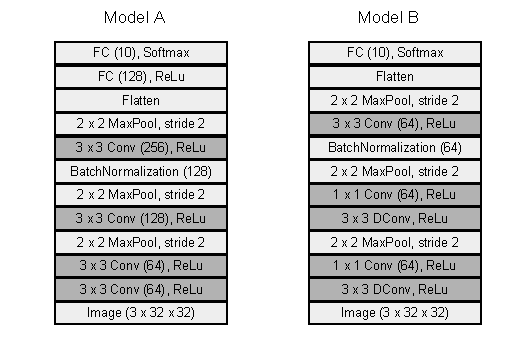
\includegraphics[width=0.5\textwidth]{../figures/models.pdf}
	\caption{CNN-based models for case study.}
	\label{fig:models}
\end{figure}

\subsection{Hardware implementations}
\begin{enumerate}
\item{Fixed-point}: To evaluate the compute performance on fixed-point, we convert $A$ and $B$ to TF Lite models with 8-bit fixed-point quantization. The compute performance is presented in \tab{tab:performance_fixed_point}. A runtime execution of $A$ is illustrated in \fig{fig:sched_model_a_fixed}. This implementation achieves a peak acceleration of $45.23\times$ in model $A$ at the tensor operation \emph{(4A) Conv}, see \tab{tab:performance_fixed_point}.

\item{Floating-point LogiCORE}: To evaluate the compute performance on floating-point models, we convert $A$ and $B$ to TF Lite without quantization. The compute performance is presented in \tab{tab:performace_float_logicore}.
This implementation achieves a peak acceleration of $9.77\times$ in model $A$ at the tensor operation \emph{(4A) Conv}.

\item{Hybrid custom floating-point approximation}: This implementation presents a peak acceleration of $44.87\times$ in model $A$ at the tensor operation \emph{(4A) Conv}. See \tab{tab:performace_float_hybrid}. This implementation achieves a $4.59\times$ acceleration over the LogiCORE floating-point implementation. The runtime execution of model $B$ with \emph{DConv} tensor operations is illustrated in \fig{fig:sched_model_b_float}.

\item{Hybrid logarithmic approximation}: This implementation is presented for comparison in \fig{fig:sched_model_a_float}, which shows the runtime executions of model $A$ with the proposed floating-point solutions including hybrid logarithmic approximation.
\end{enumerate}

\begin{table}[!htp]\centering
	\caption{Compute performance with fixed-point on model $A$ and $B$.}\label{tab:performance_fixed_point}
	\scriptsize
\begin{tabular}{lrrrrrrr}\toprule
	\multicolumn{2}{c}{\textbf{Tensor operation}} &\textbf{CPU} &\multicolumn{3}{c}{\textbf{TP (fixed-point)}} &\multirow{2}{*}{\textbf{Accel.}} \\\cmidrule{1-6}
	\textbf{Operation} &\textbf{MOP} &\textbf{t (ms)} &\textbf{t (ms)} &\textbf{MOP/s} &\textbf{GOP/W} & \\\midrule
	\multicolumn{2}{c}{\textbf{Model $A$}} & & & & & \\
	(1A) Conv &1.769 &700.22 &55.19 &32.06 &0.23 &\textbf{12.69} \\
	(2A) Conv &37.748 &12,666.91 &297.08 &127.06 &0.93 &\textbf{42.64} \\
	(3A) Conv &18.874 &6,081.01 &142.99 &131.99 &0.97 &\textbf{42.53} \\
	(4A) Conv &18.874 &5,543.77 &122.58 &153.97 &1.13 &\textbf{45.23} & \\\midrule
	\multicolumn{2}{c}{\textbf{Model $B$}} & & & & & \\
	(1B) DConv &0.027 &13.43 &0.63 &43.74 &0.25 &\textbf{21.25} \\
	(2B) Conv &0.196 &129.95 &11.57 &16.98 &0.12 &\textbf{11.23} \\
	(3B) DConv &0.147 &69.18 &3.33 &44.26 &0.25 &\textbf{20.77} \\
	(4B) Conv &1.048 &378.78 &9.96 &105.25 &0.77 &\textbf{38.02} \\
	(5B) Conv &2.359 &694.60 &16.46 &143.22 &1.05 &\textbf{42.20} \\
	\bottomrule
\end{tabular}
\end{table}

\begin{figure}[t!]
	\centering
	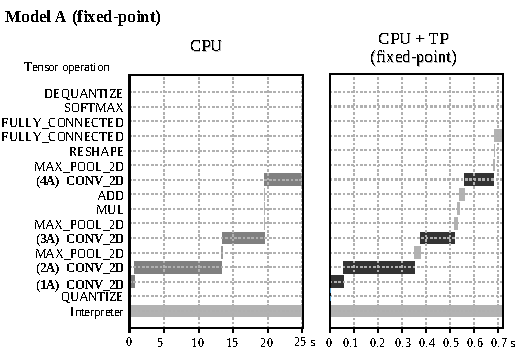
\includegraphics[width=0.5\textwidth]{../figures/sched_A_fixed_point.pdf}
	\caption{Compute performance with fixed-point on model $A$.}
	\label{fig:sched_model_a_fixed}
\end{figure}


\begin{table}[!htp]\centering
	\caption{Compute performance with floating-point LogiCORE on models $A$ and $B$.}\label{tab:performace_float_logicore}
	\scriptsize
	\begin{tabular}{lrrrrrrr}\toprule
		\multicolumn{2}{c}{\textbf{Tensor operation}} &\textbf{CPU} &\multicolumn{3}{c}{\textbf{TP (floating-point LogiCORE)}} &\multirow{2}{*}{\textbf{Accel.}} \\\cmidrule{1-6}
		\textbf{Operation} &\textbf{MOP} &\textbf{t (ms)} &\textbf{t (ms)} &\textbf{MOP/s} &\textbf{GOP/W} & \\\midrule
		\multicolumn{2}{c}{\textbf{Model $A$}} & & & & & \\
		(1A) Conv &1.769 &670.95 &120.07 &14.73 &0.21 &\textbf{5.59} \\
		(2A) Conv &37.748 &12,722.13 &1,328.08 &28.42 &0.40 &\textbf{9.58} \\
		(3A) Conv &18.874 &6,094.85 &636.53 &29.65 &0.42 &\textbf{9.58} \\
		(4A) Conv &18.874 &5,564.79 &569.30 &33.15 &0.47 &\textbf{9.77} & \\\midrule
		\multicolumn{2}{c}{\textbf{Model $B$}} & & & & & \\
		(1B) DConv &0.027 &11.51 &1.557 &17.75 &0.23 &\textbf{7.39} \\
		(2B) Conv &0.196 &94.82 &20.487 &9.59 &0.13 &\textbf{4.62} \\
		(3B) DConv &0.147 &58.84 &8.355 &17.64 &0.23 &\textbf{7.04} \\
		(4B) Conv &1.048 &368.66 &40.271 &26.03 &0.37 &\textbf{9.15} \\
		(5B) Conv &2.359 &697.08 &72.981 &32.32 &0.46 &\textbf{9.55} \\
		\bottomrule
	\end{tabular}
\end{table}

\begin{table}[!htp]\centering
	\caption{Compute performance with hybrid custom floating-point approximation on models $A$ and $B$.}\label{tab:performace_float_hybrid}
	\scriptsize
\begin{tabular}{lrrrrrrr}\toprule
	\multicolumn{2}{c}{\textbf{Tensor operation}} &\textbf{CPU} &\multicolumn{3}{c}{\textbf{TP (H. custom floating-point)}} &\multirow{2}{*}{\textbf{Accel.}} \\\cmidrule{1-6}
	\textbf{Operation} &\textbf{MOP} &\textbf{t (ms)} &\textbf{t (ms)} &\textbf{MOP/s} &\textbf{GOP/W} & \\\midrule
	\multicolumn{2}{c}{\textbf{Model $A$}} & & & & & \\
	(1A) Conv &1.769 &670.95 &68.50 &25.83 &0.39 &\textbf{9.8} \\
	(2A) Conv &37.748 &12,722.13 &307.83 &122.63 &1.85 &\textbf{41.33} \\
	(3A) Conv &18.874 &6,094.85 &147.97 &127.55 &1.93 &\textbf{41.19} \\
	(4A) Conv &18.874 &5,564.79 &124.03 &152.17 &2.30 &\textbf{44.87} & \\\midrule
	\multicolumn{2}{c}{\textbf{Model $B$}} & & & & & \\
	(1B) DConv &0.027 &11.51 &1.41 &19.63 &0.27 &\textbf{8.17} \\
	(2B) Conv &0.196 &94.82 &20.34 &9.43 &0.14 &\textbf{4.66} \\
	(3B) DConv &0.147 &58.84 &6.58 &22.41 &0.31 &\textbf{8.94} \\
	(4B) Conv &1.048 &368.66 &12.75 &82.23 &1.24 &\textbf{28.91} \\
	(5B) Conv &2.359 &697.08 &17.14 &137.68 &2.08 &\textbf{40.68} \\
	\bottomrule
\end{tabular}
\end{table}


\begin{figure*}[t!]
	\centering
	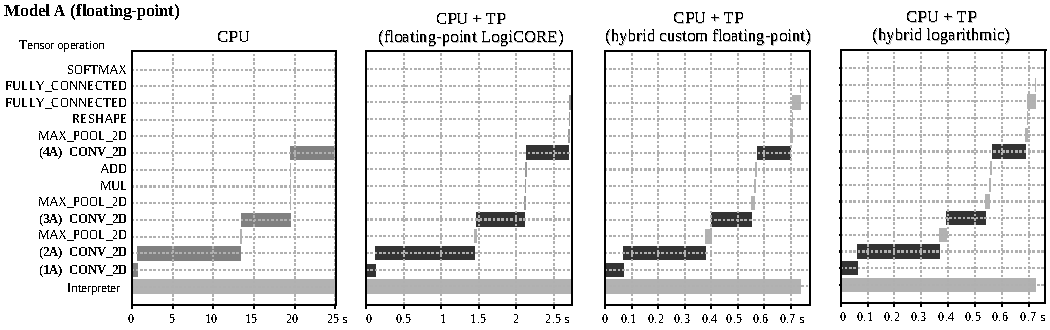
\includegraphics[width=\textwidth]{../figures/sched_A_float_all.pdf}
	\caption{Compute performance with the proposed floating-point solutions on model $A$.}
	\label{fig:sched_model_a_float}
\end{figure*}


\begin{figure}[t!]
	\centering
	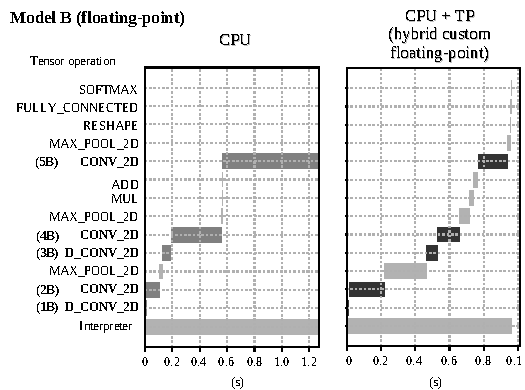
\includegraphics[width=0.5\textwidth]{../figures/sched_B_float.pdf}
	\caption{Compute performance on model $B$ (floating-point).}
	\label{fig:sched_model_b_float}
\end{figure}

\subsection{Classification accuracy}

We evaluate the classification accuracy of the CNN models under the effects of custom floating and logarithmic quantization. \tab{tab:formats} presents the list of custom formats proposed for evaluation. In this case, the \emph{filter} and \emph{bias} tensors are quantized from base floating-point representation (IEEE 754) into custom reduced formats with bit-truncation and -rounding methods. For this evaluation, we train $A$ an $B$ for image classification with CIFAR-10 dataset. We deploy the models with a baseline accuracy of 76.6\% for $A$, and 68.8\% for $B$. See \fig{fig:accuracy}.

\begin{table}[!htp]\centering
	\caption{Implemented floating-point formats for accuracy evaluation.}\label{tab:formats}
	\scriptsize
	\begin{tabular}{lrrrrr}\toprule
		\multicolumn{5}{c}{\textbf{Floating-point formats}} \\\cmidrule{1-5}
		\textbf{Name} &\textbf{Size (bits)} &\textbf{Sign} &\textbf{Exponent} &\textbf{Mantissa} \\\midrule
		Logarithmic &6 &1 &5 &0 \\
		S1-E5-M1 &7 &1 &5 &1 \\
		S1-E5-M2 &8 &1 &5 &2 \\
		S1-E5-M3 &9 &1 &5 &3 \\
		S1-E5-M4 &10 &1 &5 &4 \\
		Float16 &16 &1 &5 &10 \\
		BFloat16 &16 &1 &8 &7 \\
		Tensor Float &19 &1 &8 &10 \\
		Float32 &32 &1 &8 &23 \\
		\bottomrule
	\end{tabular}
\end{table}

\begin{figure}[t!]
	\centering
	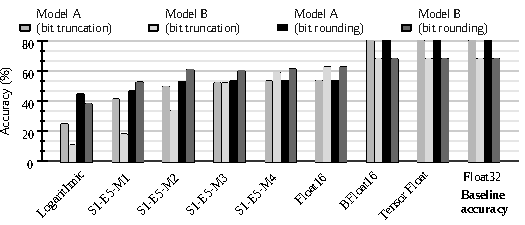
\includegraphics[width=0.5\textwidth]{../figures/all_models_accuracy.pdf}
	\caption{Accuracy performance using hybrid custom floating-point approximation with various formats. Samples: CIFAR-10 test dataset ($10,000$ images).}
	\label{fig:accuracy}
\end{figure}

\subsection{Resource utilization and power dissipation}
The resource utilization and power dissipation of the TP is listed in \tab{tab:resource}. The power dissipation of the Zynq device is presented in \fig{fig:power}. 

\begin{table}[!htp]\centering
	\caption{Resource utilization and power dissipation of the proposed TP engines.}\label{tab:resource}
	\scriptsize
\begin{tabular}{lrrrrrr}\toprule
	\textbf{} &\multicolumn{4}{c}{\textbf{Post-implementation resource utilization}} &\multirow{2}{*}{\textbf{Power (W)}} \\\cmidrule{2-5}
	\textbf{TP engine} &\textbf{LUT} &\textbf{FF} &\textbf{DSP} &\textbf{BRAM 18K} & \\\midrule
	\multicolumn{6}{l}{\textbf{1) Fixed-point}} \\
	Conv &5,677 &4,238 &78 &70 &0.136 \\
	DConv &7,232 &5,565 &106 &70 &0.171 \\
	Conv + DConv &12,684 &8,015 &160 &70 &0.248 & \\\midrule
	\multicolumn{6}{l}{\textbf{2) Floating-point LogiCore}} \\
	Conv &4,670 &3,909 &59 &266 &0.070 \\
	DConv &6,263 &5,264 &82 &266 &0.075 \\
	Conv + DConv &10,871 &7,726 &123 &266 &0.119 \\\midrule
	\multicolumn{6}{l}{\textbf{3 ) Hybrid custom floating-point approximation}} \\
	Conv &6,787 &4,349 &56 &74 &0.066 \\
	DConv &8,209 &5,592 &79 &74 &0.072 \\
	Conv + DConv &14,590 &8,494 &117 &74 &0.108 & \\\midrule
	\multicolumn{6}{l}{\textbf{4) Hybrid logarithmic approximation}} \\
	Conv &6,662 &4,242 &54 &58 &0.060 \\
	DConv &8,110 &5,380 &77 &58 &0.066 \\
	Conv + DConv &14,370 &8,175 &113 &58 &0.105 \\
	\bottomrule
\end{tabular}
\end{table}

\begin{figure}[t!]
	\centering
	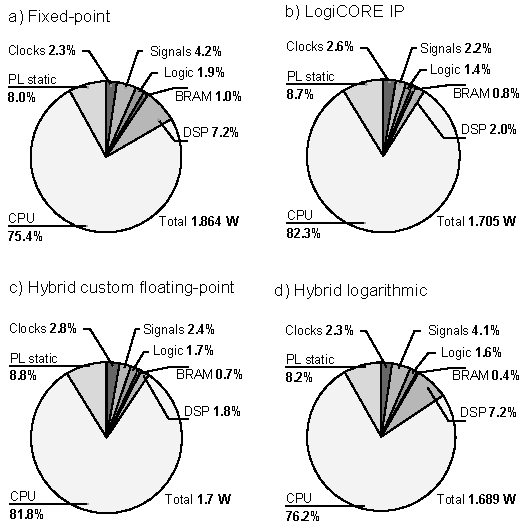
\includegraphics[width=0.5\textwidth]{../figures/power_breackdown.pdf}
	\caption{Estimated power dissipation of the Zynq-7020 SoC with different TP engines.}
	\label{fig:power}
\end{figure}


\subsection{Discussion}
\begin{enumerate}
	\item{Performance}: The dot-product with hybrid custom floating-point approximation achieves better performance with larger vectors. Since \emph{DConv} performs a channel-wise spatial dot-product, this implementation presents very limited acceleration compared with the LogiCORE-based implementation.

	One critical problem is that the computation throughput may not well match the memory bandwidth provided an FPGA platform. Consequently, existing approaches cannot achieve best performance due to underutilization of either logic resource or memory bandwidth.

	It means that the performance is degraded due to under-utilization of either logic resource or memory bandwidth.
	
	\item{Energy}: The implementations with hybrid custom floating-point and logarithmic approximation are the most efficient with energy reduction of $954\times$ and $1,055\times$, respectively. \tab{tab:edp} presents the energy-delay product (EDP) and energy reduction in \emph{(4A) Conv} operator.
	
\begin{table}[!htp]\centering
	\caption{Energy consumption in tensor operation \emph{(4A) Conv}.}\label{tab:edp}
	\scriptsize
	\begin{tabular}{lrrrrr}\toprule
		\textbf{Engine} & \textbf{t (ms)} &\textbf{Power (W)} &\textbf{EDP (J)} &\textbf{Reduction} \\\midrule
		CPU &5,564.79 &1.404 &7,812.97 &1.00 \\
		Fixed-point &122.58 &0.136 &16.67 &468.66 \\
		Floating-point LogiCORE &569.30 &0.070 &39.85 &196.05 \\
		Hybrid custom floating-point &124.03 &0.066 &8.19 &\textbf{954.43} \\
		Hybrid logarithmic &123.32 &0.060 &7.40 &\textbf{1,055.92 }\\
		\bottomrule
	\end{tabular}
\end{table}
	
	\item{Resource utilization}: In the case of fixed-point implementation, the TP includes additional logic to support the quantized multiplier and shifter channel-wise corrections implemented for TF Lite 8-bit quantization. This TP presents the highest power dissipation.
	
	\item{Accuracy}: Based on the presented classification accuracy, the hybrid custom floating-point approximation presents the best trade off between QoR and energy-efficiency.
	
	Theres is no accuracy degradation when using fixed-point and floating-point LogiCORE IP.

	\item{Functionality}: Higher energy efficiency, fast development round, and capability of reconfiguration.

	There are a lot of potential solutions that result in a huge design space for exploration
	An integration with other optional layers, such as sub-sampling or max pooling layers, will be studied in future work.
\end{enumerate}